\chapter{Results and Analysis}\label{Sect:results}
\par The quality of fit for a single model is given in fig. \ref{outputExample}. For some models, there are predictions that differ significantly, more than 100eV, from their true values, these are configurations that are difficult for the model to predict. In those cases, the number of outlying crystals has been counted then excluded from the average error calculation. In this way, the average error can become mostly independent of the model's outliers. When a difficult-to-predict configuration is poorly predicted and thus excluded from the average error, it can reduce the overall average error for a given model. A better trained model may then predict that configuration energy slightly better, within 100eV of its true value, resulting in a larger average error. Therefore the average error and number of large errors must both be considered when assessing the value of the model. 

\begin{figure}%[h]
\centering
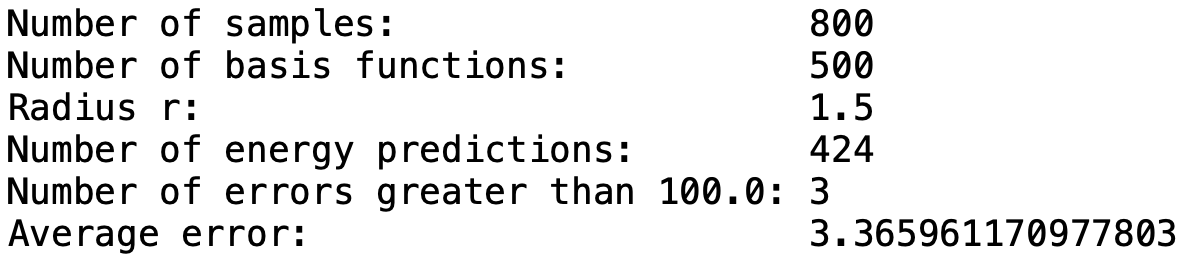
\includegraphics[scale = 0.6]{Figures/outputExample}
\caption{An example of the data in the output file generated on the supercomputer. The text gives the size of the training set, number of basis functions, and the cutoff radius used to generate the model. It also tells the size of the holdout set, the average error, and the number of errors larger than 100eV.
\label{outputExample}} 
\end{figure}

\par To understand a given model's accuracy and precision visually, each prediction energy can be plotted against the actual energy for each configuration. The model referenced in fig. \ref{outputExample} can be seen in this format in fig. \ref{accuracyPlot}.

\begin{figure}%[h]
\centering
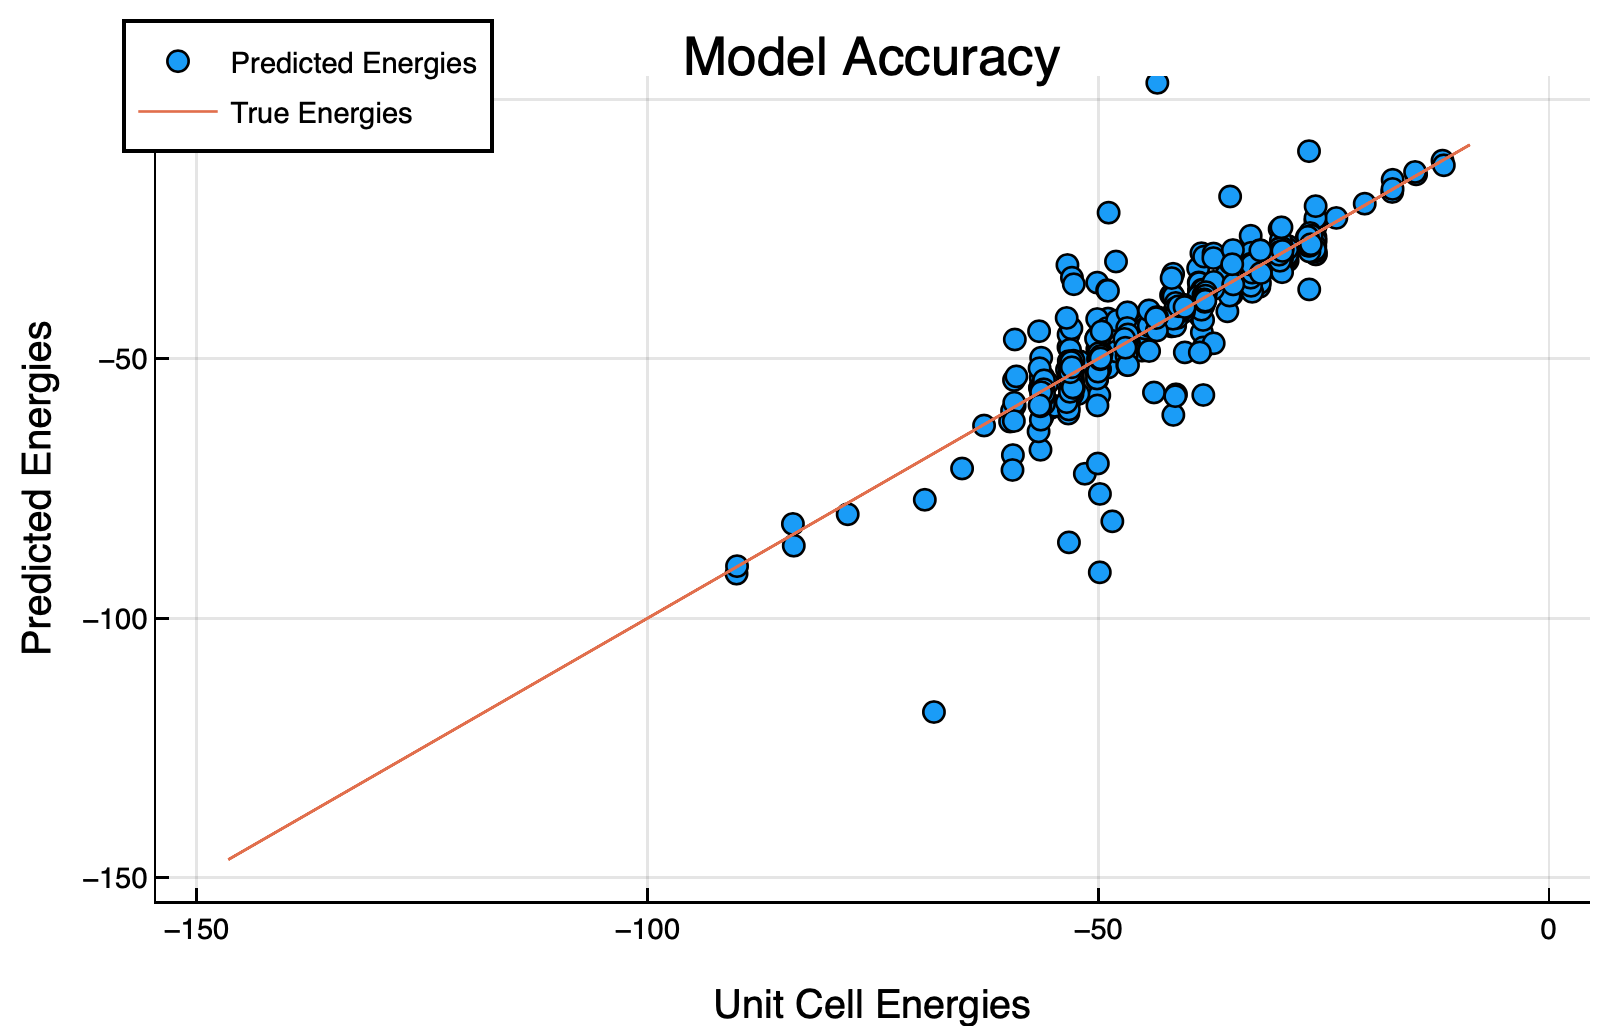
\includegraphics[scale = 0.5]{Figures/accuracyPlot}
\caption{Predicted energies versus the actual energies for each configuration in the holdout set. This model is the same as the one shown in fig. \ref{outputExample}. The prediction energies seem to form an adequate match to their true values. When the simplicity of this model is contrasted with the high levels of complexity it is attempting to capture, the accuracy of this fit is impressive.
\label{accuracyPlot}} 
\end{figure}

\par This method of visual analysis in fig. \ref{accuracyPlot} works very well for observing one model at a time but interpreting each of the 270 unique models this way would be difficult and time consuming. Preferably, several data sets could be interpreted at one time.
\par One of many possible solutions is to use a series of heatmaps showing the average error of each model with it's respective parameters. But as discussed above, the average error does not tell the whole story; the number of large errors must also be accounted for. Because the size of the holdout set changes from model to model, it would be more useful to display the percentage of large errors rather than just the number of large errros. Fig. \ref{aveErrorHeatmaps} shows five heatmaps, one for each size of training set. The color in each square represents the average error for a specific model. The scale for each subplot is set to be identical to make its analysis easier. A similar cluster of plots can be seen in fig. \ref{perErrorHeatmaps}, showing the number of large errors for each model. 

\begin{figure*}
  \centering
  \begin{subfigure}{0.5\textwidth}
    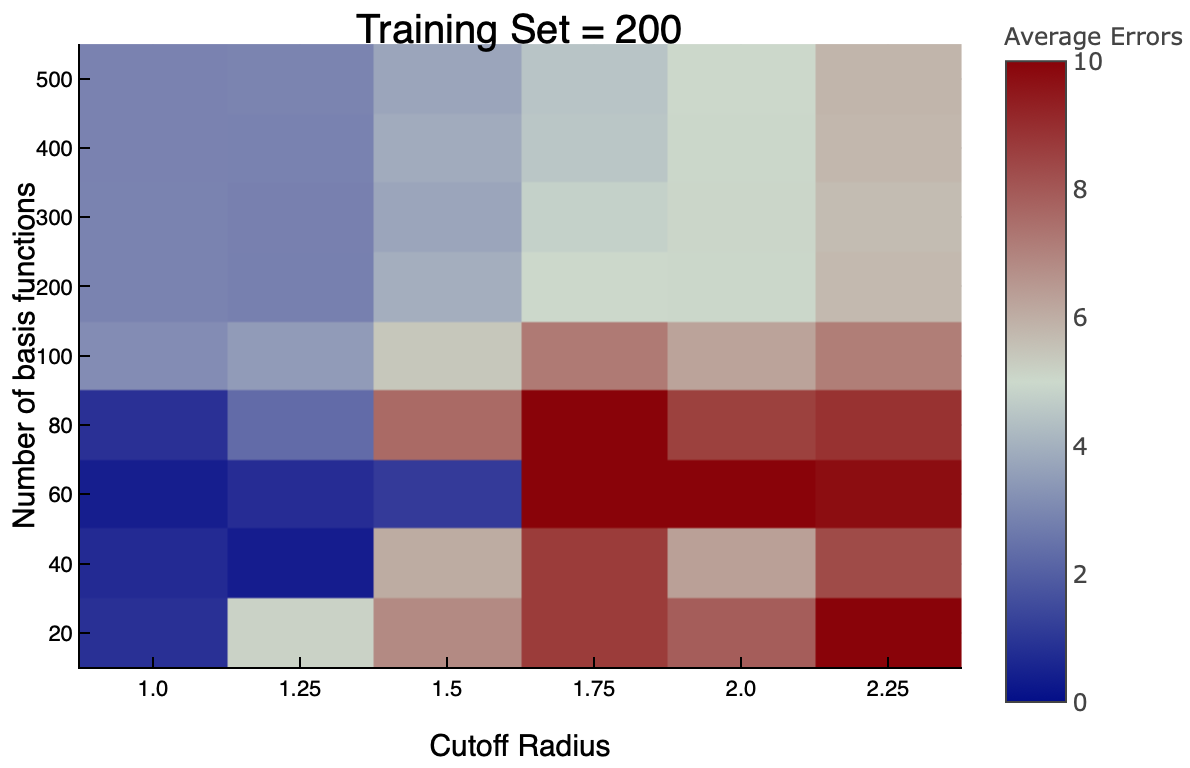
\includegraphics[width=\linewidth]{Figures/aveErrors2}
    \caption{} 
    \label{aveErrors2}
  \end{subfigure}%
  \hspace*{\fill}   % maximize separation between the subfigures
  \begin{subfigure}{0.5\textwidth}
    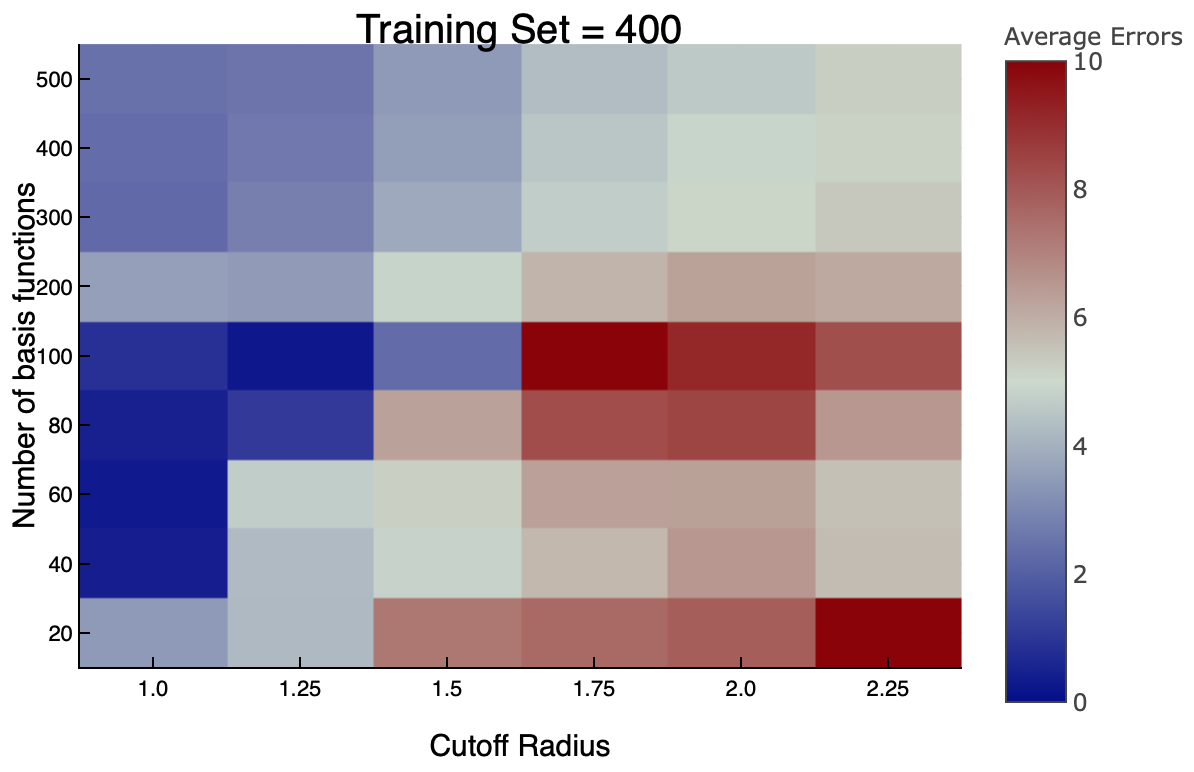
\includegraphics[width=\linewidth]{Figures/aveErrors4}
    \caption{} 
    \label{aveErrors4}
  \end{subfigure}%
    %\hspace*{\fill}   % maximize separation between the subfigures
    \\
  \begin{subfigure}{0.5\textwidth}
    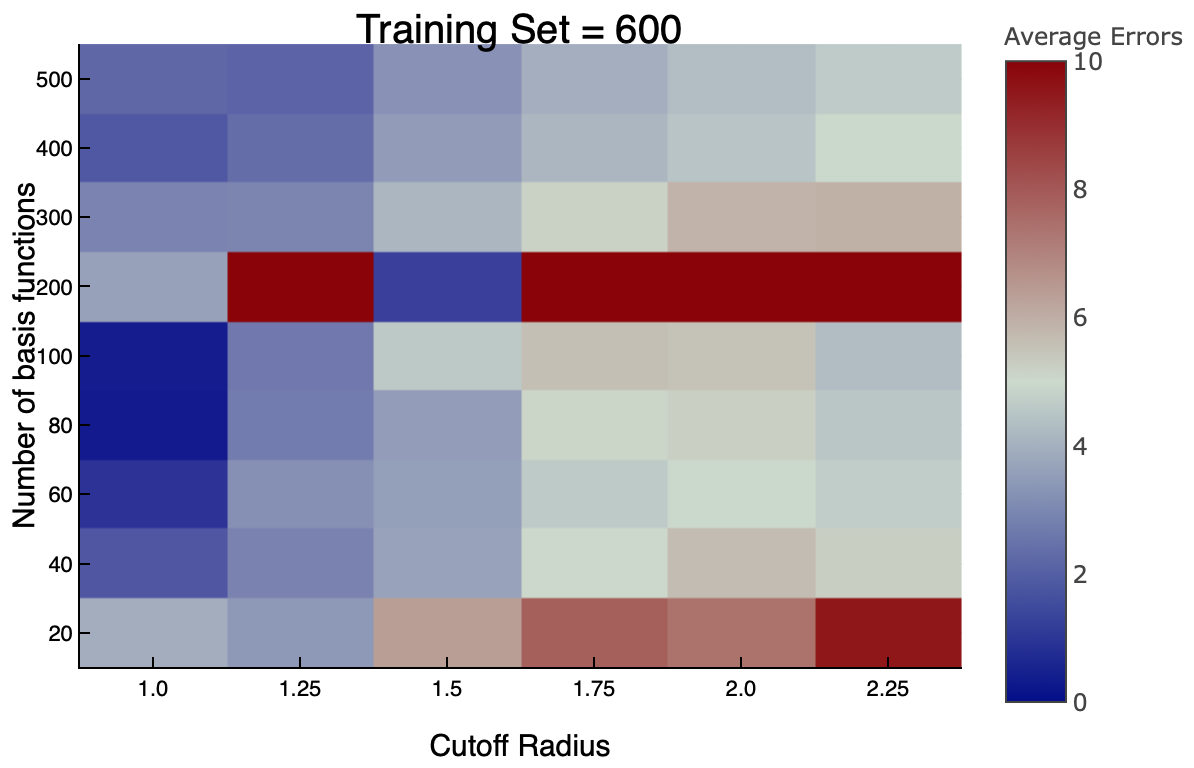
\includegraphics[width=\linewidth]{Figures/aveErrors6}
    \caption{} 
    \label{aveErrors6}
  \end{subfigure}%
    \hspace*{\fill}   % maximize separation between the subfigures
  \begin{subfigure}{0.5\textwidth}
    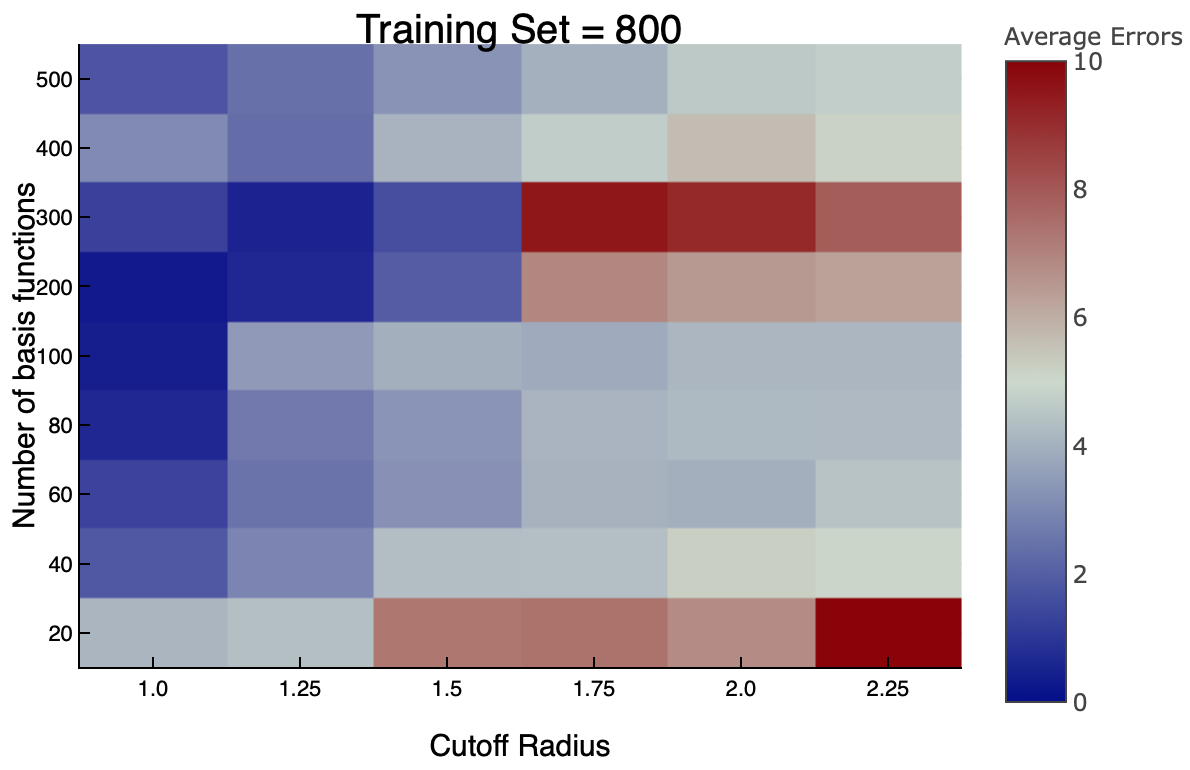
\includegraphics[width=\linewidth]{Figures/aveErrors8}
    \caption{} 
    \label{aveErrors8}
  \end{subfigure}%
    %\hspace*{\fill}   % maximize separation between the subfigures
    \\
  \begin{subfigure}{0.5\textwidth}
    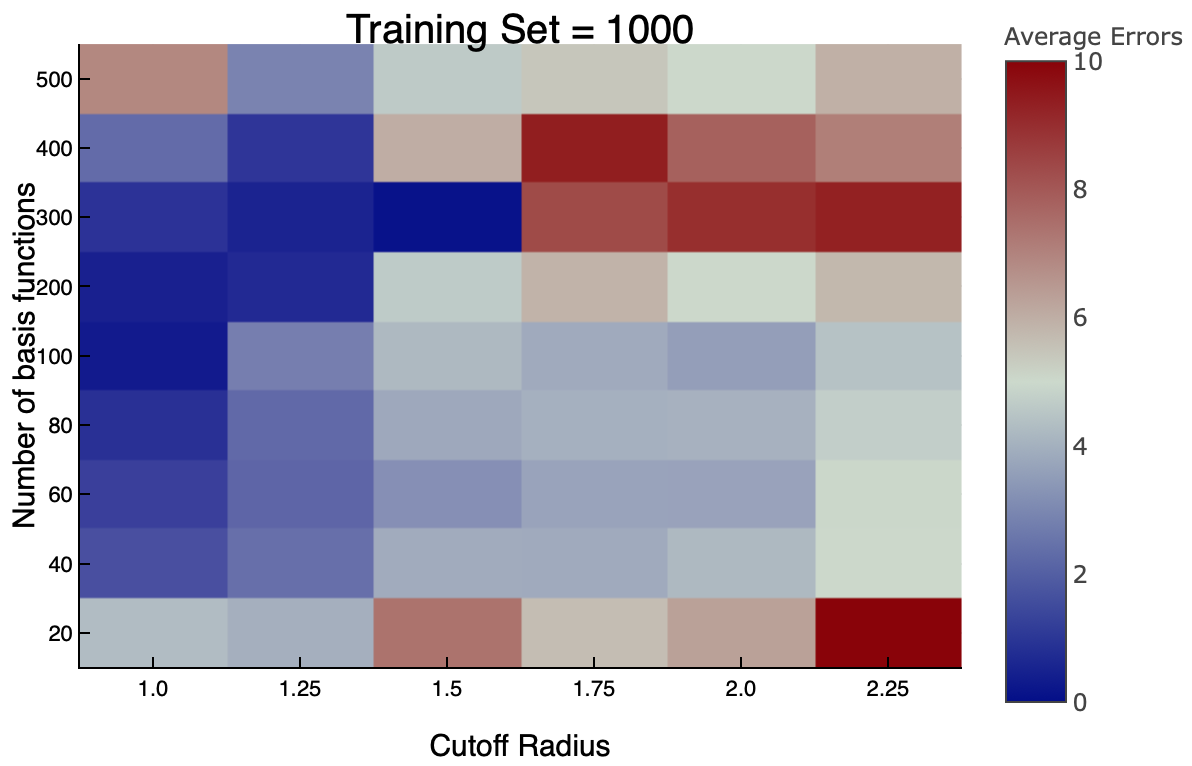
\includegraphics[width=\linewidth]{Figures/aveErrors10}
    \caption{} 
    \label{aveErrors10}
  \end{subfigure}%
\caption{Heatmaps showing the average error of each model produced. The scale for each is fixed from 0eV to 10eV. The general trend is that each plot is more blue on the left and red on the right. This is because many of the less sophisticated models predict the more difficult configurations poorly, causing them to be excluded from the average error. As the sophistication of the model increases, it will predict these configurations with greater accuracy and thus raise the average error by a noticeable amount. This can be verified by comparing these heatmaps with those in fig. \ref{perErrorHeatmaps}.
\label{aveErrorHeatmaps}}
\end{figure*}


\begin{figure*}
  \centering
  \begin{subfigure}{0.5\textwidth}
    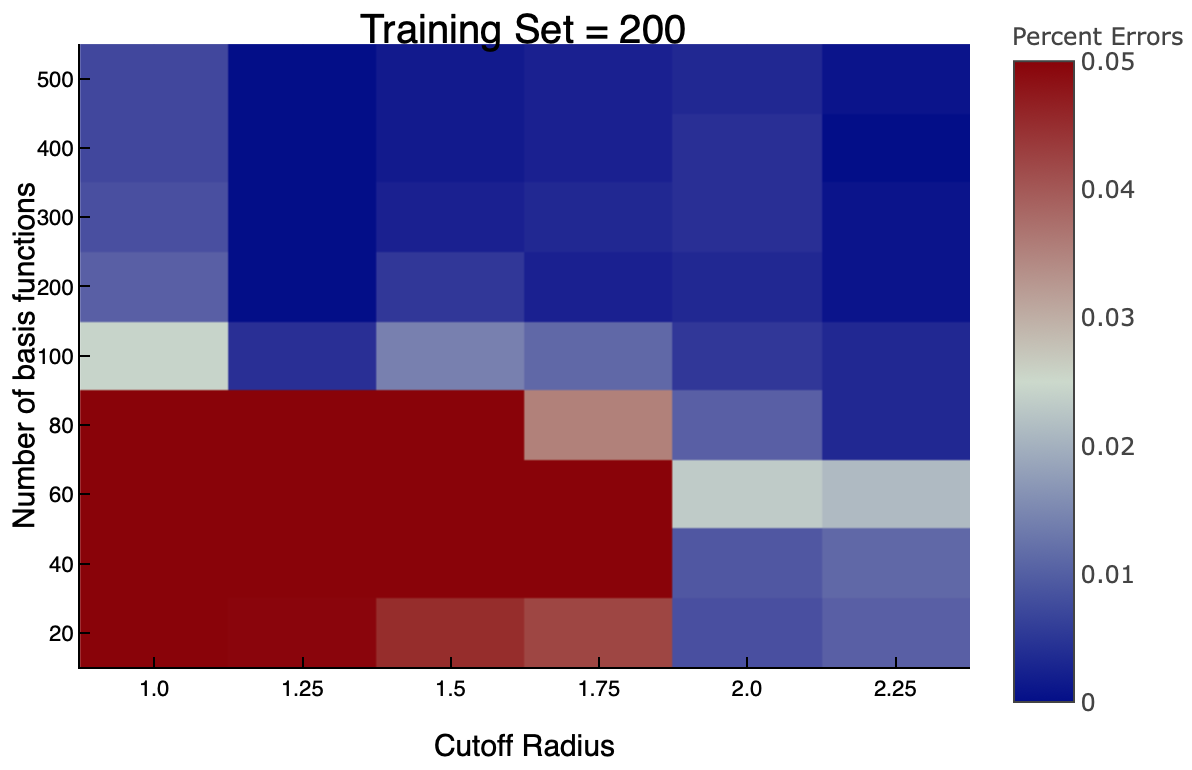
\includegraphics[width=\linewidth]{Figures/perErrors2}
    \caption{} 
    \label{perErrors2}
  \end{subfigure}%
  \hspace*{\fill}   % maximize separation between the subfigures
  \begin{subfigure}{0.5\textwidth}
    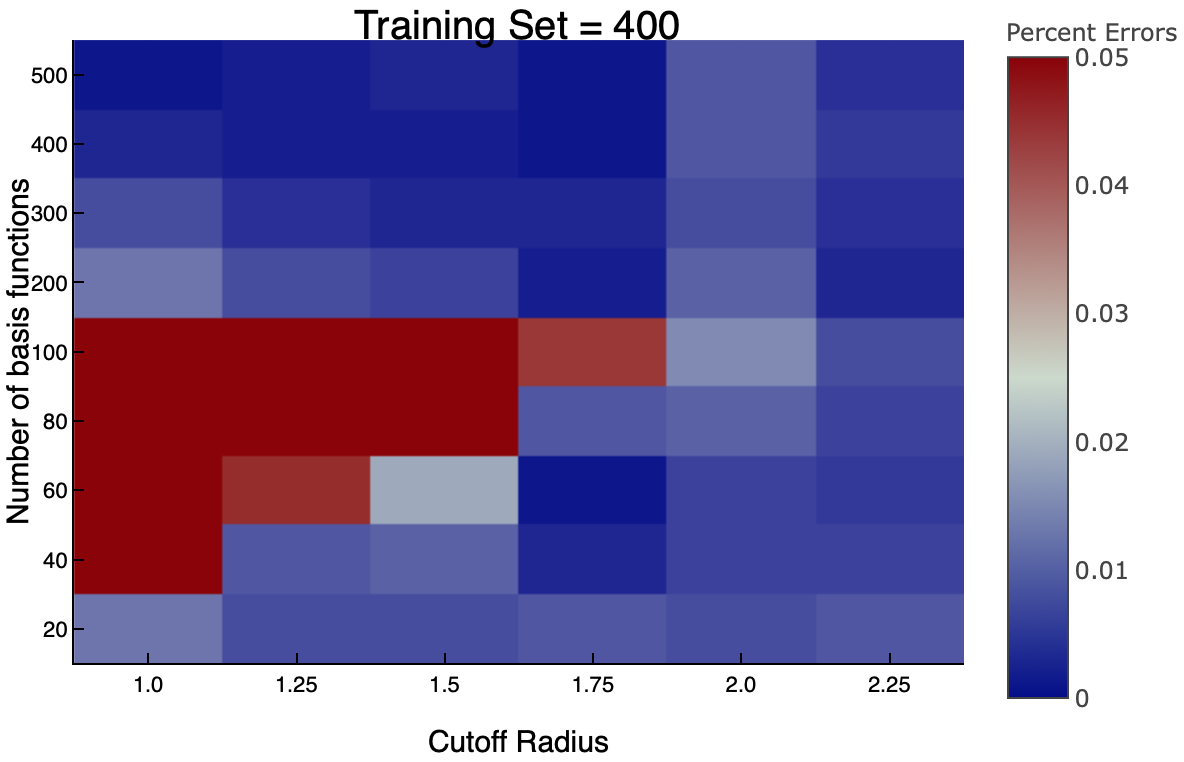
\includegraphics[width=\linewidth]{Figures/perErrors4}
    \caption{} 
    \label{perErrors4}
  \end{subfigure}%
    %\hspace*{\fill}   % maximize separation between the subfigures
    \\
  \begin{subfigure}{0.5\textwidth}
    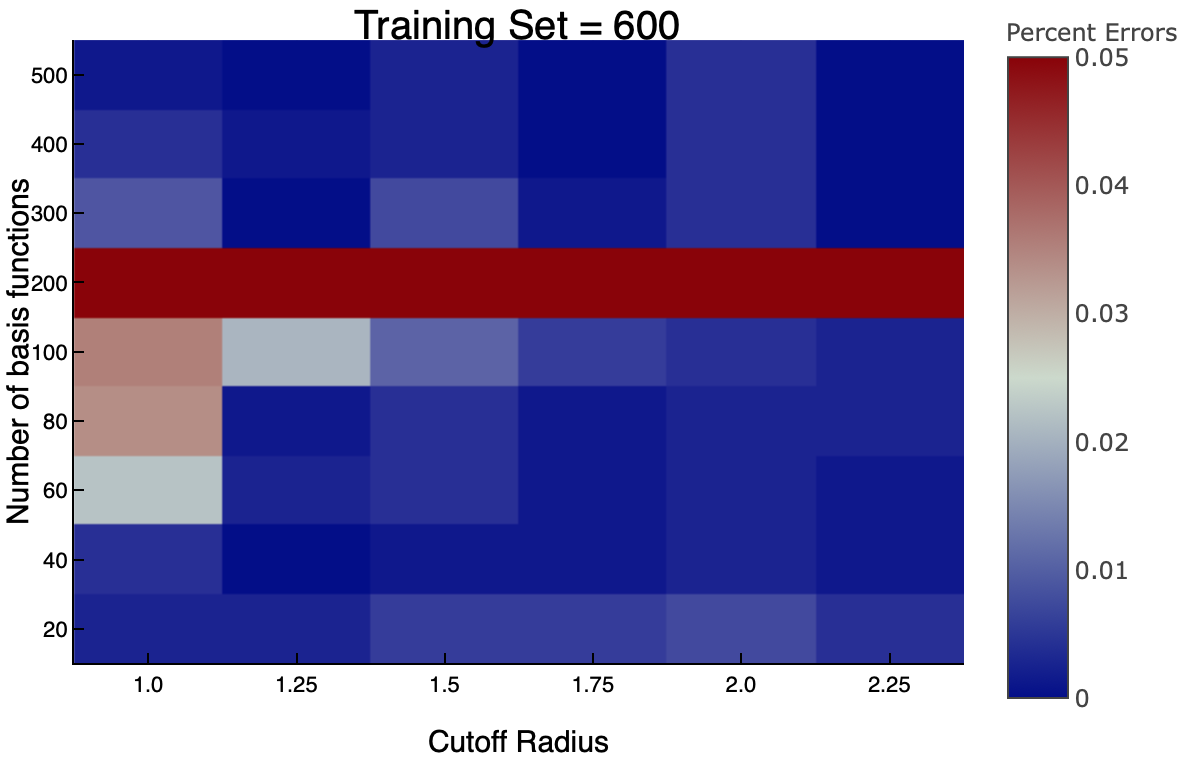
\includegraphics[width=\linewidth]{Figures/perErrors6}
    \caption{} 
    \label{perErrors6}
  \end{subfigure}%
    \hspace*{\fill}   % maximize separation between the subfigures
  \begin{subfigure}{0.5\textwidth}
    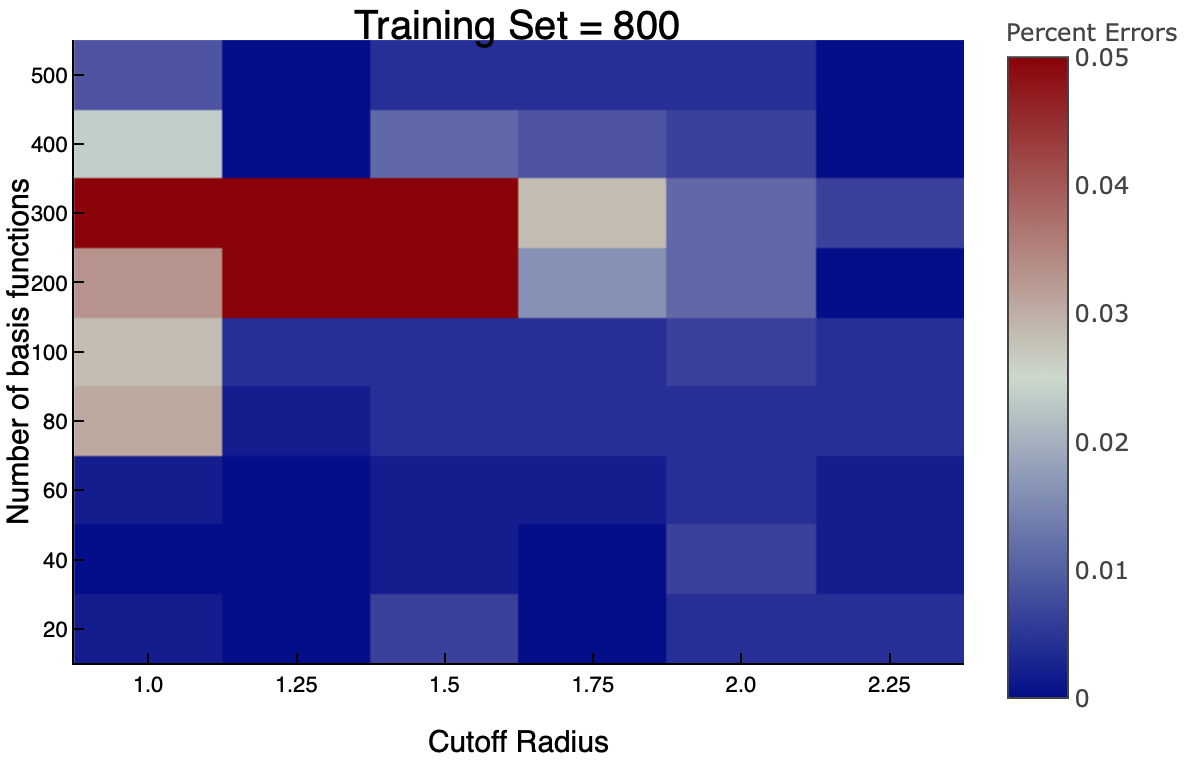
\includegraphics[width=\linewidth]{Figures/perErrors8}
    \caption{} 
    \label{perErrors8}
  \end{subfigure}%
    %\hspace*{\fill}   % maximize separation between the subfigures
    \\
  \begin{subfigure}{0.5\textwidth}
    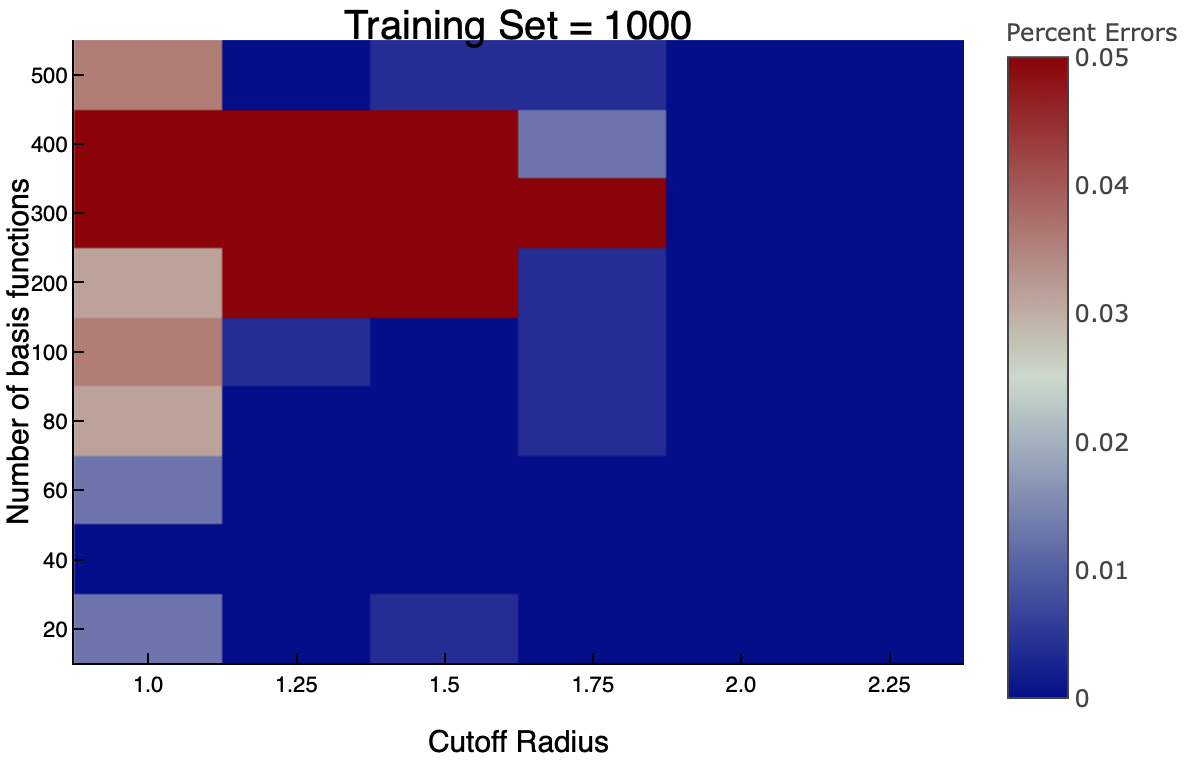
\includegraphics[width=\linewidth]{Figures/perErrors10}
    \caption{} 
    \label{perErrors10}
  \end{subfigure}%
\caption{Heatmaps showing the percentage of large errors of each model produced. The scale for each is fixed from 0-0.05, or 0-5\%. A model with a percent error of 0.01 would mean that 1 out of every 100 predictions has an error greater than 100eV. The percent error is preferred over the number of large errors because it takes into account the fact that as the size of the training set increases, the size of the holdout set decreses. Thus a model with a large training set will naturally have a smaller number of large errors, but not necessarily a smaller percentage of large errors.
\label{perErrorHeatmaps}}
\end{figure*}


\par The true accuracy and precision of each model can only be realized when comparing the results from fig. \ref{aveErrorHeatmaps} \textit{and} fig. \ref{perErrorHeatmaps}. One without the other does not show the full picture. For example, the lower left corner of fig. \ref{aveErrors2} appears to be surprisingly accurate, but when compared with the corresponding squares in fig. \ref{perErrors2}, a considerable percent of large errors can be seen. These particular models are not of interest. The models that \textit{are} of interest will be the squares from corresponding subplots in fig. \ref{aveErrorHeatmaps} and fig. \ref{perErrorHeatmaps} that are both blue or blue-ish. 
%\par fig. \ref{numErrors2} includes a large red clump in the bottom right of the plot. This red patch then appears to move upward in each ensuing figure. \ldots \ldots \ldots
\par The most successful model was trained on 1000 configurations, used 40 basis functions, and had an effective radius of 1.0. This model produced 0 large errors and had an average error of only 1.77eV. As expected, the second and third best models had very similar input parameters.
